% !TeX encoding = UTF-8
% !TeX program = xelatex
\documentclass[12pt, a4paper]{article}
\usepackage{xeCJK} % 须放在\usepackage{}列中足够前的位置
\usepackage{fontspec}
\usepackage{graphicx}
\usepackage{caption}
\usepackage{enumerate}
\usepackage{setspace}
\usepackage{array} % 製作表格必須的宏包
\usepackage{tabularx} % 自動調整列寬的表格宏包
\usepackage{adjustbox}
\setCJKfamilyfont{heiti}{Heiti TC}
\CJKfamily{heiti}
\setmainfont{Arial}
\setstretch{1.5}


\begin{document}
\begin{center}
  {\Huge 邏輯設計實驗} \\[2.5cm]
  {\Huge Lab11} \\[1.5cm]
  {\Huge 移位暫存器與應用} \\ [4.5cm]
  \hspace{.6in}
  \begin{minipage}[t]{.4\linewidth}
    {\Large 班級:資訊一甲}\\[0.5cm]
    {\Large 學號:D1109023}\\[0.5cm]
    {\Large 姓名:楊孟憲}
  \end{minipage}    
\end{center}

\newpage
%\fontsize{30pt}{36pt}\selectfont 
%\normalsize

\begin{description}
  \fontsize{22pt}{25pt}\selectfont 
    \item [一、]摘要 
      \begin{enumerate}
        \fontsize{20pt}{22pt}\selectfont
          \item 位移暫存器
            \begin{description}
              \fontsize{16pt}{20}\selectfont
                \item [(1)] 串列輸入/串列輸出(SISO)
                \item [(2)] 串列輸入/並列輸出(SIPO)
                \item [(3)] 並列輸入/並列輸出(PIPO)
                \item [(4)] 並列輸入/串列輸出(PISO)\\
              \normalsize
            \end{description}
            
              \item 實驗 
              \begin{description}
                \fontsize{16pt}{20}\selectfont
                  \item [(1)] Ring-counter 設計 LEDs交互閃爍的電路
                  \item [(2)] 6-bit可變花樣的左右旋轉跑馬燈 \\
                \normalsize  
              \end{description}

        \normalsize
      \end{enumerate}
    \item [二、]實驗結果
      \begin{description}
        \fontsize{20pt}{22pt}\selectfont
        \item 實驗一
          \fontsize{16pt}{18pt}\selectfont
            \begin{description}
              \item [$\bullet$]利用 Ring-counter,設計一個LEDs交互閃爍的電路
              \item [$\bullet$]按下Reset鍵時, Ring-counter最左邊的DFF會被preset,其餘的DFF會被reset.
              \item [$\bullet$]當Start = 1時, 每按一次Clock, LEDs變換左右閃爍 \\[.2cm]
              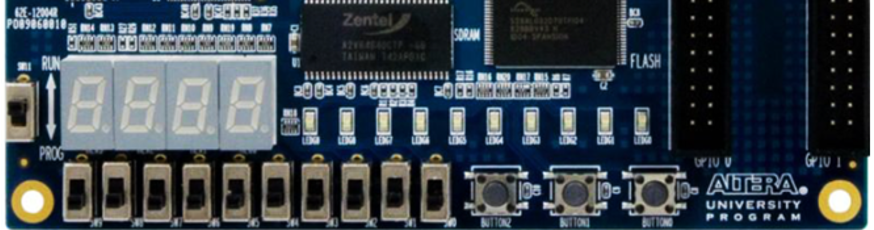
\includegraphics[width=10cm]{./image/ex1_sample.png}
                \item[$\bullet$] 實作想法 \\
                    \begin{samepage}
                        當 start = 1 時,按下 click 鈕,會讓跑馬燈左右跳動。\\
                        首先使用暫存器將 click 狀態儲存起來,並且利用 not 和 and 閘 切換當前狀態。(左右跳動)\\
                    \end{samepage}
                  \fontsize{18pt}{20pt}
                  \item [(1)]電路圖 \\[.3cm]
                  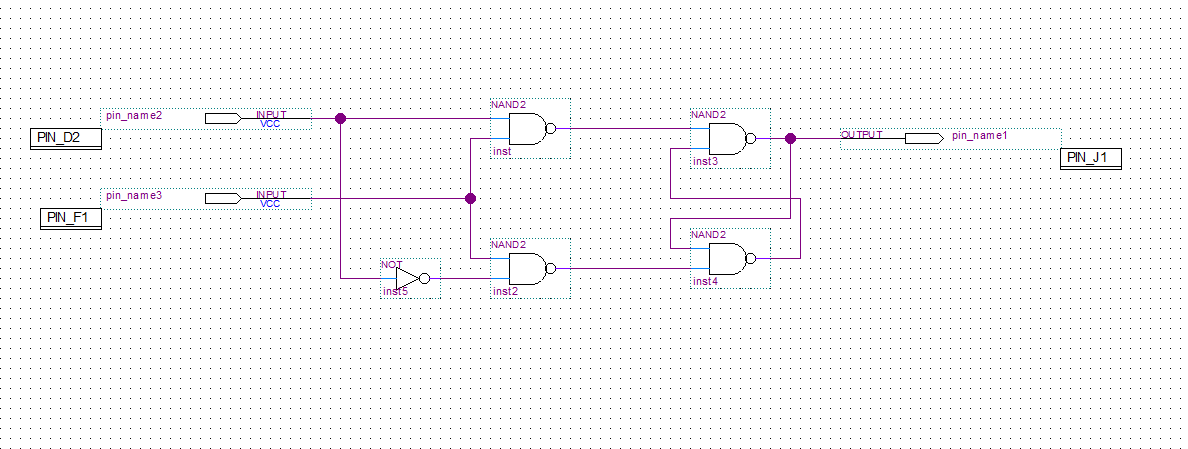
\includegraphics[width=13cm]{./image/ex1.PNG}
                \item [(2)] 波形圖 \\[.3cm]
                  \includegraphics[width=13cm]{./image/eX1_1.PNG}  \\          
            \end{description}
          \normalsize
          
          \fontsize{20pt}{22pt}\selectfont
          \item 實驗二
          \fontsize{16pt}{18pt}\selectfont
            \begin{description}
              \item [$\bullet$] 設計一個6-bit可變花樣的左右旋轉跑馬燈
              \item [$\bullet$] 輸入 $F_{0}$、$F_{1}$ 並使用多工器判斷要做的事。 \\
                
\includegraphics[width=7cm]{./image/ex2_4to1.png}
              \fontsize{18pt}{20pt}
                \item [(1)]電路圖 \\[.3cm]
                  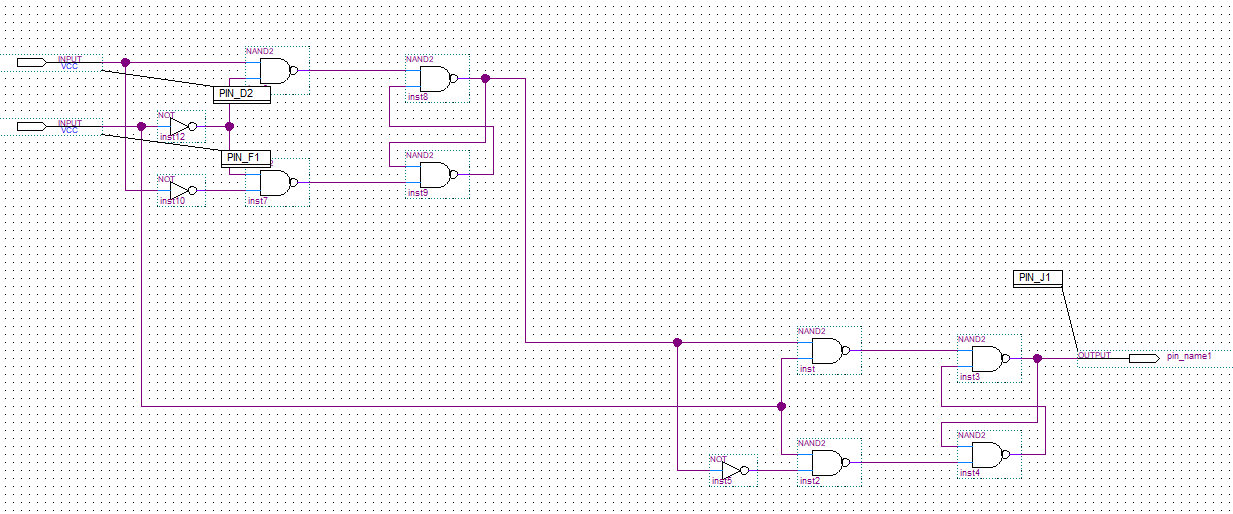
\includegraphics[width=13cm]{./image/ex2.PNG} \\
            \end{description}
          \normalsize
        \normalsize
      \end{description}
    \item [三、]問題討論心得 \\[.6cm]
      \begin{minipage}[t]{\linewidth}
        \fontsize{16}{18}\selectfont
            這次的實驗實作暫存器的使用,利用上週教的 latch 結合 not 和 and 閘,來實現訊號暫存,當按鈕按下,將訊號切換並且站存起來。
            我覺得在設計邏輯閘上有越來越上手了,時做出實驗也越來越有成就感,很快就能想到要如何設計。但隨著題目難度提升,在接線的方面也要更加小心。
        \normalsize  
      \end{minipage}
  \normalsize
\end{description}

\end{document}


